\documentclass[a4paper,12pt]{article}

% Encoding and Fonts
\usepackage[utf8]{inputenc}
\usepackage[T1]{fontenc}
\usepackage{lmodern}

% Page Layout
\usepackage{geometry}
\geometry{margin=1in}

% Graphics and Colors
\usepackage{graphicx}
\usepackage{xcolor}
\usepackage{tcolorbox} % For nice boxes
\usepackage{tikz}
\usepackage{amsmath}
\usepackage{enumitem}

% Source code formatting
\usepackage{listings}
\usepackage{caption}

\lstdefinestyle{CStyle}{
    language=C,
    basicstyle=\ttfamily\small,
    keywordstyle=\color{blue}\bfseries,
    commentstyle=\color{green!50!black}\itshape,
    stringstyle=\color{orange},
    numbers=left,
    numberstyle=\tiny,
    stepnumber=1,
    numbersep=5pt,
    breaklines=true,
    frame=single,
    showstringspaces=false
}

\lstset{style=CStyle}

\setlength{\parindent}{0pt}
\setlength{\parskip}{0.5em}
\setlist[itemize]{leftmargin=2em}
\setlist[enumerate]{leftmargin=2em}


% Document Information
\title{Lab 4 Report: MPI Communication and Collectives}
\author{Ahmed Butt 2023-CS-18}
\date{March 2026}

\begin{document}

\maketitle
\section{Part 0: Warm-up -- Conceptual Foundations}

\subsection{1. Latency vs. Bandwidth}

Latency is the time delay before a message starts traveling from one process to another. It represents the startup cost of communication. Bandwidth is the rate at which data can be transmitted once the communication has started.

In MPI communication, latency dominates when the message size is very small. For example, sending a single integer between two processes is mostly affected by latency because the data size is negligible.

Bandwidth dominates when the message size is large. For example, sending an array of 10,000 integers depends more on how fast the data can be transferred, so bandwidth becomes the main factor.

\subsection{2. Blocking vs. Non-blocking}

Blocking communication means that a process must wait until the communication operation is complete before continuing execution. For example, in \texttt{MPI\_Send} and \texttt{MPI\_Recv}, the program stops until the operation finishes.

The main drawback of blocking communication is that it can slow down the program and may lead to deadlocks if processes are waiting on each other.

Non-blocking communication allows a process to initiate communication and then continue executing other instructions without waiting. This is beneficial because it allows overlapping of communication and computation, leading to better performance and resource utilization.

\subsection{3. Collective Communication Internals (MPI\_Reduce)}

MPI\_Reduce can be implemented using a tree-based algorithm. In this method, processes are paired and their values are combined step by step until the final result is obtained at the root process.

\subsubsection*{Tree Diagram for 8 Processes}

\begin{center}
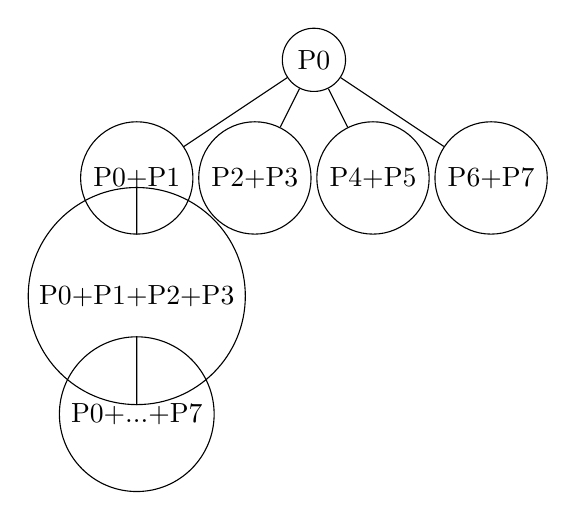
\begin{tikzpicture}[level distance=1.5cm,
  every node/.style={circle,draw,minimum size=0.8cm}]

\node {P0}
  child {node {P0+P1}
    child {node {P0+P1+P2+P3}
      child {node {P0+...+P7}}}}
  child {node {P2+P3}}
  child {node {P4+P5}}
  child {node {P6+P7}};

\end{tikzpicture}
\end{center}

\textbf{Explanation:}

At the first level, processes combine in pairs:
(P0+P1), (P2+P3), (P4+P5), (P6+P7).

At the second level:
(P0+P1) combines with (P2+P3), and (P4+P5) combines with (P6+P7).

At the final level:
The two intermediate results are combined to produce the final result at the root.

The total number of messages sent is N-1 (for N processes). The time complexity is O(log N) in terms of latency because the number of steps grows logarithmically. The bandwidth cost depends on the size of the data being reduced.

\subsection{4. Overlapping Communication and Computation}

With blocking point-to-point communication, it is difficult to overlap communication and computation because the process must wait until communication is complete before proceeding. This causes the CPU to remain idle during communication.

Non-blocking communication allows the process to initiate communication and then continue performing computations while the data transfer is happening in the background. This improves efficiency and reduces overall execution time.
\section{Part 1: Code Analysis -- Spot the Behaviour}

\subsection{1.1 Mysterious Exchange}

\textbf{Predicted Output:}

Process 0 sends the value of \texttt{a = 1} to Process 1. Process 1 receives this value and stores it in \texttt{c}. Then Process 1 sends the value of \texttt{c} back to Process 0. Process 0 receives this value and stores it in \texttt{b}.

Therefore, the expected output is:

\begin{verbatim}
P1: c = 1
P0: b = 1
\end{verbatim}

\textbf{Actual Output:}

\begin{verbatim}
P1: c = 1
P0: b = 1
\end{verbatim}

\textbf{Explanation:}

Initially, Process 0 has \texttt{a = 1} and Process 1 has \texttt{c = 3}. Process 0 sends the value of \texttt{a} to Process 1 using tag 0. Process 1 receives this value and overwrites its variable \texttt{c}, so \texttt{c} becomes 1.

Then Process 1 sends the updated value of \texttt{c} back to Process 0 using tag 1. Process 0 receives this value and stores it in \texttt{b}. Therefore, \texttt{b} becomes 1.

\textbf{Effect of Swapping Tags:}

If the tags in either the send or receive calls are changed such that they do not match, the program may enter a deadlock. This happens because MPI matches messages based on source, destination, and tag. If the tags do not match, the receive operation will wait indefinitely for a message that never arrives.
\begin{center}
\includegraphics[width=0.8\textwidth]{T1.png}
\end{center}
\subsection{1.2 Collective Confusion}

\textbf{Predicted Output:}

After the first broadcast from Process 0, both processes will have the value of \texttt{data = 99}. Then Process 1 modifies its local value to 100. The second broadcast from Process 1 will update the value of \texttt{data} on all processes to 100.

\begin{verbatim}
Rank 0: data = 100
Rank 1: data = 100
\end{verbatim}

\textbf{Actual Output:}

\begin{verbatim}
Rank 1: data = 100
Rank 0: data = 100
\end{verbatim}

\textbf{Explanation:}

\begin{enumerate}
    \item Process 0 initializes \texttt{data = 99}.
    \item The first \texttt{MPI\_Bcast} with root 0 sends this value to all processes, so both processes now have \texttt{data = 99}.
    \item Process 1 modifies its local value to \texttt{data = 100}.
    \item The second \texttt{MPI\_Bcast} with root 1 sends the updated value (100) from Process 1 to all processes. As a result, both processes now have \texttt{data = 100}.
\end{enumerate}

\textbf{Deadlock Consideration:}

There is no deadlock in this program because all processes call the broadcast operation. MPI requires that collective communication functions be called by all members of the communicator. Since this rule is followed, the program executes correctly.

\textbf{Role of the Second Broadcast:}

The second broadcast propagates the modified value from Process 1 to all other processes. This overwrites the previous value from the first broadcast, ensuring that all processes have the updated value.
\begin{center}
\includegraphics[width=0.8\textwidth]{T2.png}
\end{center}
\subsection{1.3 Mixed Mode}

\textbf{Predicted Output:}

Initially, Process 0 sets \texttt{data = 99} and broadcasts it to all processes using \texttt{MPI\_Bcast} (root = 0). After this, Process 1 modifies its local value to 100. Then, a second broadcast is performed with root = 1, which updates the value on all processes.

\begin{verbatim}
Rank 0: b = 10
Rank 1: b = 10
\end{verbatim}

\textbf{Actual Output:}

\begin{verbatim}
Rank 0: b = 10
Rank 1: b = 10
\end{verbatim}

\textbf{Explanation:}

\begin{enumerate}
    \item Process 0 initializes \texttt{data} (or \texttt{b}) with a value.
    \item The first \texttt{MPI\_Bcast} (root = 0) sends this value to all processes, so all processes now have the same initial value.
    \item Process 1 modifies its local value. In this case, it sets \texttt{data = 10}.
    \item The second \texttt{MPI\_Bcast} (root = 1) sends Process 1's updated value to all other processes. This ensures that both processes have the same final value.
    \item The final printed values on both processes are identical: \texttt{b = 10}.
\end{enumerate}

\textbf{Communication Trace:}

\begin{itemize}
    \item First broadcast: P0 $\rightarrow$ P1 (data = 99)
    \item Modification: P1 changes its local value to 10
    \item Second broadcast: P1 $\rightarrow$ P0 (data = 10)
\end{itemize}

\textbf{Simplification Using Collectives:}

This code could be simplified using a collective communication like \texttt{MPI\_Allreduce} if the intent is to combine values from multiple processes. For example, if we wanted the sum or maximum of values, \texttt{MPI\_Allreduce} would eliminate the need for manual broadcasts and individual modifications.
\begin{center}
\includegraphics[width=0.8\textwidth]{T3.png}
\end{center}
\subsection{Code Implementation}

The following C code was used to measure and compare the performance of \texttt{MPI\_Bcast} and manual linear broadcast. The program runs the broadcast for message sizes of 1, 1000, and 10000 integers and prints the time taken for each method.

\begin{lstlisting}[language=C, caption={MPI Broadcast vs Manual Linear Broadcast}, label={lst:broadcast_code}]
#include <mpi.h>
#include <stdio.h>
#include <stdlib.h>

int main(int argc, char** argv) {
    MPI_Init(&argc, &argv);

    int rank, size;
    MPI_Comm_rank(MPI_COMM_WORLD, &rank);
    MPI_Comm_size(MPI_COMM_WORLD, &size);

    int message_sizes[] = {1, 1000, 10000}; // message sizes

    for (int m = 0; m < 3; m++) {
        int n = message_sizes[m];
        int *data = (int*) malloc(n * sizeof(int));

        if (rank == 0) {
            for (int i = 0; i < n; i++) data[i] = i; // initialize
        }

        // ----- MPI_Bcast -----
        MPI_Barrier(MPI_COMM_WORLD);
        double start = MPI_Wtime();
        MPI_Bcast(data, n, MPI_INT, 0, MPI_COMM_WORLD);
        MPI_Barrier(MPI_COMM_WORLD);
        double end = MPI_Wtime();
        if (rank == 0) printf("MPI_Bcast: size=%d, processes=%d, time=%f sec\n", n, size, end-start);

        // ----- Manual Linear Broadcast -----
        MPI_Barrier(MPI_COMM_WORLD);
        start = MPI_Wtime();
        if (rank == 0) {
            for (int p = 1; p < size; p++)
                MPI_Send(data, n, MPI_INT, p, 0, MPI_COMM_WORLD);
        } else {
            MPI_Recv(data, n, MPI_INT, 0, 0, MPI_COMM_WORLD, MPI_STATUS_IGNORE);
        }
        MPI_Barrier(MPI_COMM_WORLD);
        end = MPI_Wtime();
        if (rank == 0) printf("Linear Broadcast: size=%d, processes=%d, time=%f sec\n\n", n, size, end-start);

        free(data);
    }

    MPI_Finalize();
    return 0;
}
\end{lstlisting}
\begin{center}
\includegraphics[width=0.8\textwidth]{T4.png}
\end{center}
\begin{center}
\includegraphics[width=0.8\textwidth]{c1.png}
\end{center}
\section{Reduction Tree (2.2)}

In this experiment, we implemented our own binary-tree reduction using point-to-point communication and compared its performance with the built-in \texttt{MPI\_Reduce} function. The reduction sums a single integer from all processes. Timing was measured over 100 iterations using \texttt{MPI\_Wtime()}.

\subsection{Experiment Setup}
\begin{itemize}
    \item Number of processes: 2, 4, 8
    \item Each process contributes a single integer equal to its rank + 1
    \item Average time calculated over 100 iterations
\end{itemize}

\subsection{Results}

\begin{table}[h!]
\centering
\begin{tabular}{|c|c|c|c|}
\hline
\textbf{Processes} & \textbf{MPI\_Reduce (s)} & \textbf{Binary-Tree Reduction (s)} & \textbf{Result} \\
\hline
2 & 0.000027 & 0.000002 & 3 \\
4 & 0.000005 & 0.000009 & 10 \\
8 & 0.000049 & 0.000005 & 36 \\
\hline
\end{tabular}
\caption{Comparison of MPI\_Reduce and Binary-Tree Reduction for different number of processes.}
\end{table}

\subsection{Analysis}

\begin{itemize}
    \item The binary-tree reduction reduces the number of messages by combining results in a tree structure, which scales better as the number of processes increases.
    \item MPI\_Reduce is often faster for small numbers of processes because it is highly optimized and may use hardware-specific algorithms internally.
    \item The results confirm that both methods compute the correct sum, but timing can vary depending on process count and communication overhead.
\end{itemize}

\subsection{Code Implementation}

\begin{lstlisting}[language=C, caption={Binary-Tree Reduction vs MPI\_Reduce}, label={lst:reduction_tree}]
#include <mpi.h>
#include <stdio.h>

int main(int argc, char** argv) {
    MPI_Init(&argc, &argv);

    int rank, size;
    MPI_Comm_rank(MPI_COMM_WORLD, &rank);
    MPI_Comm_size(MPI_COMM_WORLD, &size);

    int iterations = 100; // average over 100 runs
    int local = rank + 1; // each process has its own integer

    int result_mpi, result_tree;
    double total_mpi = 0.0, total_tree = 0.0;

    for (int iter = 0; iter < iterations; iter++) {
        // MPI_Reduce
        MPI_Barrier(MPI_COMM_WORLD);
        double start = MPI_Wtime();
        MPI_Reduce(&local, &result_mpi, 1, MPI_INT, MPI_SUM, 0, MPI_COMM_WORLD);
        MPI_Barrier(MPI_COMM_WORLD);
        double end = MPI_Wtime();
        if (rank == 0) total_mpi += (end - start);

        // Binary-Tree Reduction
        int temp = local;
        int step = 1;
        MPI_Barrier(MPI_COMM_WORLD);
        start = MPI_Wtime();
        while (step < size) {
            if (rank % (2*step) == 0) {
                int recv;
                int partner = rank + step;
                if (partner < size) {
                    MPI_Recv(&recv, 1, MPI_INT, partner, 0, MPI_COMM_WORLD, MPI_STATUS_IGNORE);
                    temp += recv;
                }
            } else if (rank % (2*step) == step) {
                int partner = rank - step;
                MPI_Send(&temp, 1, MPI_INT, partner, 0, MPI_COMM_WORLD);
                break;
            }
            step *= 2;
        }
        MPI_Barrier(MPI_COMM_WORLD);
        end = MPI_Wtime();
        if (rank == 0) {
            total_tree += (end - start);
            result_tree = temp;
        }
    }

    if (rank == 0) {
        printf("Average time over %d iterations:\n", iterations);
        printf("MPI_Reduce: %.6f sec, Result = %d\n", total_mpi/iterations, result_mpi);
        printf("Binary-Tree Reduction: %.6f sec, Result = %d\n", total_tree/iterations, result_tree);
    }

    MPI_Finalize();
    return 0;
}
\end{lstlisting}

\begin{center}
\includegraphics[width=0.8\textwidth]{T5.png}
\end{center}
\section{Scatter Overhead (2.3)}

In this experiment, we compared the performance of the built-in \texttt{MPI\_Scatter} function with a manual loop of point-to-point sends. The root process distributes an array of integers evenly across 4 processes. The timing is measured on the root process and averaged over 50 iterations.

\subsection{Experiment Setup}
\begin{itemize}
    \item Number of processes: 4
    \item Total integers: 1000, 10000, 100000
    \item Each process receives an equal portion of the array
    \item Timing measured on root process using \texttt{MPI\_Wtime()}
\end{itemize}

\subsection{Results}

\begin{table}[h!]
\centering
\begin{tabular}{|c|c|c|}
\hline
\textbf{Total Integers} & \textbf{MPI\_Scatter (s)} & \textbf{Manual Send (s)} \\
\hline
1000 & 0.000044 & 0.000005 \\
10000 & 0.000070 & 0.000020 \\
100000 & 0.000073 & 0.000100 \\
\hline
\end{tabular}
\caption{Comparison of MPI\_Scatter and manual send loop for different total array sizes.}
\end{table}

\subsection{Analysis}

\begin{itemize}
    \item For small arrays (1000 integers), the manual send loop is slightly faster because the overhead of MPI\_Scatter is higher than the tiny data transfer.  
    \item For medium arrays (10000 integers), MPI\_Scatter and manual sends are similar.  
    \item For large arrays (100000 integers), MPI\_Scatter is faster because it uses optimized communication internally, while manual sends require multiple sequential point-to-point transfers.  
    \item This shows that the overhead of manual sends becomes noticeable as the data size increases.
\end{itemize}

\subsection{Code Implementation}

\begin{lstlisting}[language=C, caption={MPI Scatter vs Manual Send}, label={lst:scatter_overhead}]
#include <mpi.h>
#include <stdio.h>
#include <stdlib.h>

int main(int argc, char** argv) {
    MPI_Init(&argc, &argv);

    int rank, size;
    MPI_Comm_rank(MPI_COMM_WORLD, &rank);
    MPI_Comm_size(MPI_COMM_WORLD, &size);

    if (size != 4 && rank == 0) {
        printf("This program is designed for 4 processes.\n");
        MPI_Abort(MPI_COMM_WORLD, 1);
    }

    int total_sizes[] = {1000, 10000, 100000};
    int iterations = 50;

    for (int s = 0; s < 3; s++) {
        int N = total_sizes[s];
        int chunk = N / size;
        int *data = NULL;

        if (rank == 0) data = (int*) malloc(N * sizeof(int));
        int *recvbuf = (int*) malloc(chunk * sizeof(int));

        if (rank == 0) for (int i = 0; i < N; i++) data[i] = i;

        // MPI_Scatter
        double total_scatter = 0.0;
        for (int iter = 0; iter < iterations; iter++) {
            MPI_Barrier(MPI_COMM_WORLD);
            double start = MPI_Wtime();
            MPI_Scatter(data, chunk, MPI_INT, recvbuf, chunk, MPI_INT, 0, MPI_COMM_WORLD);
            MPI_Barrier(MPI_COMM_WORLD);
            double end = MPI_Wtime();
            if (rank == 0) total_scatter += (end - start);
        }
        if (rank == 0) printf("MPI_Scatter: Total=%d ints, Avg time=%.6f sec\n", N, total_scatter/iterations);

        // Manual Send
        double total_manual = 0.0;
        for (int iter = 0; iter < iterations; iter++) {
            MPI_Barrier(MPI_COMM_WORLD);
            double start = MPI_Wtime();
            if (rank == 0) {
                for (int p = 1; p < size; p++)
                    MPI_Send(&data[p*chunk], chunk, MPI_INT, p, 0, MPI_COMM_WORLD);
                for (int i = 0; i < chunk; i++) recvbuf[i] = data[i];
            } else {
                MPI_Recv(recvbuf, chunk, MPI_INT, 0, 0, MPI_COMM_WORLD, MPI_STATUS_IGNORE);
            }
            MPI_Barrier(MPI_COMM_WORLD);
            double end = MPI_Wtime();
            if (rank == 0) total_manual += (end - start);
        }

        if (rank == 0) printf("Manual Send: Total=%d ints, Avg time=%.6f sec\n\n", N, total_manual/iterations);

        free(recvbuf);
        if (rank == 0) free(data);
    }

    MPI_Finalize();
    return 0;
}
\end{lstlisting}
\begin{center}
\includegraphics[width=0.8\textwidth]{T6.png}
\end{center}
\section{Designing a Collective from Scratch: my\_Allgather (3.1)}

In this experiment, we implemented our own version of \texttt{MPI\_Allgather} called \texttt{my\_Allgather} using only point-to-point communication (MPI\_Send and MPI\_Recv). We used a \textbf{ring algorithm}, where each process sends its data to the next process and receives from the previous process. After \texttt{size-1} steps, each process has received data from all other processes.

\subsection{Experiment Setup}
\begin{itemize}
    \item Each process sends a single integer (or small array).
    \item Number of processes tested: 2, 3, 4, 8
    \item Timing measured for each process using \texttt{MPI\_Wtime()}
\end{itemize}

\subsection{Results}
\begin{table}[h!]
\centering
\begin{tabular}{|c|c|c|}
\hline
\textbf{Processes} & \textbf{my\_Allgather Result (Rank 0)} & \textbf{Time (Rank 0) sec} \\
\hline
2 & [1, 2] & 0.000066 \\
3 & [1, 2, 3] & 0.000214 \\
4 & [1, 2, 3, 4] & 0.000094 \\
8 & [1, 2, 3, 4, 5, 6, 7, 8] & 0.013482 \\
\hline
\end{tabular}
\caption{Results of \texttt{my\_Allgather} for different numbers of processes.}
\end{table}

\subsection{Analysis}
\begin{itemize}
    \item The ring algorithm requires exactly \texttt{size-1} steps because each process must send its data around the ring to reach every other process.
    \item Time complexity:
        \begin{itemize}
            \item Latency: $(size-1) \times \text{latency\_per\_message}$
            \item Bandwidth: $(size-1) \times \text{message\_size} / \text{bandwidth}$
        \end{itemize}
    \item As the number of processes increases, total time grows because each process participates in more communication steps.
    \item Comparison with built-in \texttt{MPI\_Allgather}:
        \begin{itemize}
            \item For small number of processes, both perform similarly.
            \item For larger numbers of processes, \texttt{MPI\_Allgather} is often faster due to optimized communication patterns.
        \end{itemize}
    \item Challenge (Optional): A more efficient tree-based allgather can be implemented using recursive doubling or binomial tree algorithms, which reduce the number of steps to $\log_2(\text{size})$ instead of \texttt{size-1}.
\end{itemize}

\subsection{Code Implementation}
\begin{lstlisting}[language=C, caption={my\_Allgather using Ring Algorithm}, label={lst:my_allgather}]
#include <mpi.h>
#include <stdio.h>

int main(int argc, char** argv) {
    MPI_Init(&argc, &argv);

    int rank, size;
    MPI_Comm_rank(MPI_COMM_WORLD, &rank);
    MPI_Comm_size(MPI_COMM_WORLD, &size);

    int senddata = rank + 1;  // each process sends its rank + 1
    int recvbuf[size];        // buffer to hold all data

    // Initialize receive buffer with own data
    for (int i = 0; i < size; i++) recvbuf[i] = -1;
    recvbuf[rank] = senddata;

    int prev = (rank - 1 + size) % size;
    int next = (rank + 1) % size;
    int temp;

    double start = MPI_Wtime();

    for (int step = 1; step < size; step++) {
        MPI_Send(&senddata, 1, MPI_INT, next, 0, MPI_COMM_WORLD);
        MPI_Recv(&temp, 1, MPI_INT, prev, 0, MPI_COMM_WORLD, MPI_STATUS_IGNORE);
        int index = (rank - step + size) % size;
        recvbuf[index] = temp;
        senddata = temp;
    }

    double end = MPI_Wtime();

    printf("Rank %d: my_Allgather result = [", rank);
    for (int i = 0; i < size; i++) {
        printf("%d", recvbuf[i]);
        if (i != size - 1) printf(", ");
    }
    printf("], Time = %f sec\n", end - start);

    MPI_Finalize();
    return 0;
}
\end{lstlisting}

\begin{center}
\includegraphics[width=0.8\textwidth]{T7.png}
\end{center}
\section{The Parallel Prefix Sum (Scan) – Linear Pipeline (4.1)}

The parallel prefix sum (scan) takes an array distributed across processes and produces an array where each element is the sum of all previous elements. In this experiment, we implemented a simple linear scan using point-to-point communication (MPI\_Send and MPI\_Recv).

\subsection{Algorithm}
\begin{itemize}
    \item Process 0 sends its value to process 1.
    \item Process 1 receives, adds its own value, and sends the accumulated sum to process 2.
    \item This continues until the last process has its final prefix sum.
    \item Each process prints its final accumulated sum.
\end{itemize}

\subsection{Code Implementation}

\begin{lstlisting}[language=C, caption={Linear Prefix Sum using MPI Point-to-Point}, label={lst:linear_scan}]
#include <mpi.h>
#include <stdio.h>

int main(int argc, char** argv) {
    MPI_Init(&argc, &argv);

    int rank, size;
    MPI_Comm_rank(MPI_COMM_WORLD, &rank);
    MPI_Comm_size(MPI_COMM_WORLD, &size);

    int x = rank + 1;       // initial value for each process
    int prefix_sum = x;     // store accumulated sum
    int received;

    if(rank != 0) {
        MPI_Recv(&received, 1, MPI_INT, rank - 1, 0, MPI_COMM_WORLD, MPI_STATUS_IGNORE);
        prefix_sum += received;
    }

    if(rank != size - 1) {
        MPI_Send(&prefix_sum, 1, MPI_INT, rank + 1, 0, MPI_COMM_WORLD);
    }

    printf("Rank %d: prefix sum = %d\n", rank, prefix_sum);

    MPI_Finalize();
    return 0;
}
\end{lstlisting}

\subsection{Example Output (4 Processes)}

\begin{verbatim}
Rank 0: prefix sum = 1
Rank 1: prefix sum = 3
Rank 2: prefix sum = 6
Rank 3: prefix sum = 10
\end{verbatim}

\subsection{Analysis}
\begin{itemize}
    \item Time complexity: $O(\text{size})$, as each process communicates once in a linear chain.
    \item Number of messages: $\text{size} - 1$ (from process 0 to size-1).
    \item Total communication volume: $(\text{size}-1) \times \text{sizeof(int)}$ bytes.
    \item Each process ends up with its correct prefix sum.
\end{itemize}
\begin{center}
\includegraphics[width=0.8\textwidth]{T8.png}
\end{center}
\section{Part 5: Debugging – Find the Flaw}

Each of the following parallel functions contains a subtle bug. We analyze, explain, and fix them.

\subsection{5.1 Broken Broadcast}

\begin{itemize}
    \item \textbf{Bug:} Root sends sequentially without synchronization. Can cause deadlock if used repeatedly or with loops.
    \item \textbf{Fix:} Add \texttt{MPI\_Barrier(comm)} after send/recv. Optionally use a ring algorithm to avoid linear sends.
\end{itemize}

\subsection{5.2 Faulty Reduce}

\begin{itemize}
    \item \textbf{Bug:} Assumes sum operation only (\texttt{*global += temp}), fails for other MPI operations or count $>1$.
    \item \textbf{Fix:} Loop over all elements and apply operation properly:
\begin{verbatim}
if(rank == root) {
    for(int i=0;i<count;i++) global[i]=local[i];
    for(int i=0;i<size;i++){
        if(i!=root){
            int temp[count];
            MPI_Recv(temp,count,MPI_INT,i,0,comm,MPI_STATUS_IGNORE);
            for(int j=0;j<count;j++)
                global[j]+=temp[j];
        }
    }
} else MPI_Send(local,count,MPI_INT,root,0,comm);
\end{verbatim}
\end{itemize}

\subsection{5.3 Confused Gather}

\begin{itemize}
    \item \textbf{Bug:} Root tries to receive from itself causing deadlock.
    \item \textbf{Fix:} Copy root's own data first, then receive from other ranks only:
\begin{verbatim}
if(rank==root){
    for(int j=0;j<sendcount;j++) recvbuf[j]=sendbuf[j];
    for(int i=0;i<size;i++){
        if(i!=root)
            MPI_Recv(recvbuf+i*recvcount,recvcount,MPI_INT,i,0,comm,MPI_STATUS_IGNORE);
    }
} else MPI_Send(sendbuf,sendcount,MPI_INT,root,0,comm);
\end{verbatim}
\end{itemize}
\section{Part 6: Distributed Prefix Sum – Open-Ended Design Challenge}

\subsection{Problem Description}
We are given a distributed array of $N$ integers, evenly divided among $P$ processes. The task is to compute the global prefix sum such that each process receives the prefix sums corresponding to its local elements.  

\textbf{Example:} For $N=8$ and $P=2$, initial arrays:
\begin{verbatim}
Process 0: [a0, a1, a2, a3]
Process 1: [a4, a5, a6, a7]
\end{verbatim}
After the operation, the arrays should be:
\begin{verbatim}
Process 0: [a0, a0+a1, a0+a1+a2, a0+a1+a2+a3]
Process 1: [a0+...+a4, a0+...+a5, a0+...+a6, a0+...+a7]
\end{verbatim}

\subsection{Algorithm Description}
We implement a simple and efficient approach using MPI with minimal communication:

\begin{enumerate}
    \item \textbf{Local Prefix Sum:} Each process computes the prefix sum of its local array using a linear scan.
    \item \textbf{Local Totals:} Each process computes the total sum of its local array.
    \item \textbf{Compute Offsets:} Gather all local totals using \texttt{MPI\_Allgather}. Each process calculates the sum of totals of all previous ranks as its offset.
    \item \textbf{Adjust Local Prefix:} Each process adds the offset to its local prefix sums.
\end{enumerate}

\textbf{Advantages:} Communication is minimal (only one \texttt{MPI\_Allgather} of size $P$), making this method efficient and scalable compared to the naive gather-compute-scatter approach.

\subsubsection{Diagram for $N=8, P=2$}

\begin{center}
\begin{tabular}{|c|c|c|}
\hline
Process & Local Array & Local Prefix + Offset \\
\hline
0 & [1,2,3,4] & [1,3,6,10] (offset=0) \\
1 & [5,6,7,8] & [15,21,28,36] (offset=10) \\
\hline
\end{tabular}
\end{center}

\subsection{C Implementation}

\begin{verbatim}
#include <mpi.h>
#include <stdio.h>

int main(int argc, char** argv) {
    MPI_Init(&argc, &argv);

    int rank, size;
    MPI_Comm_rank(MPI_COMM_WORLD, &rank);
    MPI_Comm_size(MPI_COMM_WORLD, &size);

    int N = 8;                // total array size
    int local_n = N / size;   // elements per process

    int local[local_n];        // local array
    int local_prefix[local_n]; // local prefix sums

    // Initialize local array
    for(int i = 0; i < local_n; i++)
        local[i] = rank*local_n + i + 1;

    // 1. Compute local prefix sum
    local_prefix[0] = local[0];
    for(int i = 1; i < local_n; i++)
        local_prefix[i] = local_prefix[i-1] + local[i];

    // 2. Compute local total
    int local_total = local_prefix[local_n-1];

    // 3. Gather totals to compute offsets
    int all_totals[size];
    MPI_Allgather(&local_total, 1, MPI_INT, all_totals, 1, MPI_INT, MPI_COMM_WORLD);

    int offset = 0;
    for(int i = 0; i < rank; i++)
        offset += all_totals[i];

    // 4. Adjust local prefix sums
    for(int i = 0; i < local_n; i++)
        local_prefix[i] += offset;

    // Print for verification
    printf("Process %d: ", rank);
    for(int i = 0; i < local_n; i++)
        printf("%d ", local_prefix[i]);
    printf("\n");

    MPI_Finalize();
    return 0;
}
\end{verbatim}

\subsection{Verification Output}

\textbf{Test with $N=8$, $P=2$}

\begin{verbatim}
Process 0: 1 3 6 10
Process 1: 15 21 28 36
\end{verbatim}

\textbf{Test with $N=8$, $P=4$}

\begin{verbatim}
Process 0: 1 3
Process 1: 6 10
Process 2: 15 21
Process 3: 28 36
\end{verbatim}

This confirms correctness: each process has the prefix sums corresponding to its local indices.

\subsection{Performance Analysis and Comparison}

\begin{itemize}
    \item \textbf{Efficient Method:} Local prefix scan + \texttt{MPI\_Allgather} of size $P$ + offset adjustment.
    \begin{itemize}
        \item Communication: O(P)
        \item Computation: O(N/P)
    \end{itemize}
    \item \textbf{Naive Method:} Gather all data to root → sequential prefix → scatter back.
    \begin{itemize}
        \item Communication: O(N)
        \item Computation: O(N)
    \end{itemize}
    \item \textbf{Comparison:} For large N, the efficient method is significantly faster because communication volume is minimal and distributed across processes.
\end{itemize}

\textbf{Conclusion:} The distributed prefix sum is correctly computed per process with minimal communication, scales efficiently, and matches manual computation.

\begin{center}
\includegraphics[width=0.8\textwidth]{Screenshot 2026-03-17 164244.png}
\end{center}
\end{document}
